
\documentclass[10pt,fleqn, twocolumn]{IEEEtran}
\usepackage{amsfonts}
\usepackage{amsthm}
\usepackage{amsmath}
\usepackage{graphicx}
\usepackage{fancyhdr}


\newtheorem{Prop}{Proposition}
\newtheorem{lemma}{Lemma}
\newtheorem{theorem}{Theorem}

\setlength{\parindent}{3em} \setlength{\oddsidemargin}{0in}
\setlength{\textwidth}{6.5in} % sets 1in left and right margins
\setlength{\topmargin}{0.20in} % change to 0.2in for regular latex
%\setlength{\headheight}{0in}
%\setlength{\footheight}{0.5in}
\setlength{\footskip}{0.5in}
\setlength{\textheight}{9.0in} %sets 1in top and bottom margins
\renewcommand{\baselinestretch}{1} %set to 1.5 for double spacing.

\newcommand{\br}{{\mathbf r}}
\newcommand{\bA}{{\mathbf A}}
\newcommand{\ba}{{\bf a}}
\newcommand{\bb}{{\bf b}}
\newcommand{\bc}{{\bf c}}
\newcommand{\bC}{{\bf C}}
\newcommand{\bd}{{\bf d}}
\newcommand{\be}{{\bf e}}
\newcommand{\bE}{{\bf E}}
\newcommand{\bbf}{{\bf f}}
\newcommand{\bF}{{\bf F}}
\newcommand{\bh}{{\bf h}}
\newcommand{\bH}{{\bf H}}
\newcommand{\bg}{{\bf g}}
\newcommand{\bG}{{\bf G}}
\newcommand{\bq}{{\bf q}}
\newcommand{\bs}{{\bf s}}
\newcommand{\bm}{{\bf m}}
\newcommand{\bn}{{\bf n}}
\newcommand{\bu}{{\bf u}}
\newcommand{\bv}{{\bf v}}
\newcommand{\bw}{{\bf w}}
\newcommand{\bx}{{\bf x}}
\newcommand{\by}{{\bf y}}
\newcommand{\bz}{{\bf z}}
\newcommand{\bL}{{\bf L}}
\newcommand{\bM}{{\bf M}}
\newcommand{\bN}{{\bf N}}
\newcommand{\bS}{{\bf S}}
\newcommand{\bT}{{\bf T}}
\newcommand{\bD}{{\bf D}}
\newcommand{\bX}{{\bf X}}
\newcommand{\bP}{{\bf P}}
\newcommand{\bQ}{{\bf Q}}
\newcommand{\bI}{{\bf I}}
\newcommand{\bR}{{\bf R}}
\newcommand{\bU}{{\bf U}}
\newcommand{\bV}{{\bf V}}
\newcommand{\bW}{{\bf W}}
\newcommand{\bY}{{\bf Y}}
\newcommand{\bZ}{{\bf Z}}
\newcommand{\bJ}{{\bf J}}
\newcommand{\bB}{{\bf B}}
\newcommand{\bzero}{{\bf 0}}
\newcommand{\bgamma}{{\mbox {\boldmath $\gamma$}}}
\newcommand{\btheta}{{\mbox {\boldmath $\theta$}}}
\newcommand{\bvartheta}{{\mbox {\boldmath $\vartheta$}}}
\newcommand{\bDelta}{{\mbox {\boldmath $\Delta$}}}
\newcommand{\bLambda}{{\mbox {\boldmath $\Lambda$}}}
\newcommand{\bPsi}{{\mbox {\boldmath $\Psi$}}}
\newcommand{\bPhi}{{\mbox {\boldmath $\Phi$}}}
\newcommand{\bcA}{{\mbox {\boldmath ${\cal A}$}}}
\newcommand{\bcB}{{\mbox {\boldmath ${\cal B}$}}}
\newcommand{\bcC}{{\mbox {\boldmath ${\cal C}$}}}
\newcommand{\bcD}{{\mbox {\boldmath ${\cal D}$}}}
\newcommand{\bcF}{{\mbox {\boldmath ${\cal F}$}}}
\newcommand{\bcG}{{\mbox {\boldmath ${\cal G}$}}}
\newcommand{\bcL}{{\mbox {\boldmath ${\cal L}$}}}
\newcommand{\bcN}{{\mbox {\boldmath ${\cal N}$}}}
\newcommand{\bcR}{{\mbox {\boldmath ${\cal R}$}}}
\newcommand{\bcS}{{\mbox {\boldmath ${\cal S}$}}}
\newcommand{\bcH}{{\mbox {\boldmath ${\cal H}$}}}
\newcommand{\bcI}{{\mbox {\boldmath ${\cal I}$}}}
\newcommand{\bcO}{{\mbox {\boldmath ${\cal O}$}}}
\newcommand{\bcP}{{\mbox {\boldmath ${\cal P}$}}}
\newcommand{\bcQ}{{\mbox {\boldmath ${\cal Q}$}}}
\newcommand{\bcV}{{\mbox {\boldmath ${\cal V}$}}}
\newcommand{\bcW}{{\mbox {\boldmath ${\cal W}$}}}


\title{Enhanced Hierarchical Modulation}
\author{\\LG Electronics Mobile Research\\San Diego, CA 92131-1807}
\date{}
\begin{document}
\maketitle
\begin{abstract}\small
Two schemes enhancing hierarchical modulation are presented and
analyzed in this paper. One scheme is to optimize the
enhancement-layer signal constellation(s) for higher spectral
efficiency. The other one is to optimize Gray bits-to-symbol
mapping for less demodulation errors. Both schemes are simple and
efficient. They can be used to recover the throughput loss of
regular hierarchical modulations with little complexity increase.
The rationales behind the proposed approaches are presented with
the analysis of achievable rate, effective signal-to-noise ratio,
modulation efficiency, Voronoi decomposition and minimum Euclidean
distance and the comparison with regular modulations. Computer
simulations are also provided to support our conclusions.
\end{abstract}
\section{Introduction}
Broadcast multicast service (BCMCS) has increasingly been popular
for delivering multimedia content to mobile users. BCMCS can be
offered through either a 3rd generation and beyond radio access
network like WCDMA or EV-DO network or a dedicate digital
broadcast infrastructure like DVB-T/H/S2, MediaFLO and DMB.
Traditional digital broadcast system is designed with the tradeoff
between maximum achievable rate and intended coverage in mind.
Their capacities are limited by maximum transmit power and worst
channel conditions so that every user in an intended coverage area
can reliably receive services. The users under good reception
condition and with advanced receiver may not have many advantages,
even though their achievable throughput can be much higher.

Recently there are lots of interests in upgrading existing digital
broadcast systems with more services for new users while keep
existing users unchanged, delivering  additional or better quality
of service (QoS) to users with advanced receivers while still
guaranteing others' services, and providing unequal protection on
digital contents~\cite{DVB,MediaFLO,Jiang05,UMB}. Many
technologies are under investigation for these goals, such as
rateless coding, hierarchical modulation, multiple-input
multiple-output (MIMO) and selective retransmission. However,
backward compatibility is one of the major concerns in upgrading
existing systems with additional service channels since there are
a large number of users already served by existing systems and it
is prohibitively expensive to simply replace their existing user
equipments by next-generation ones. It is also expected that
existing receivers can continue to operate in upgraded systems,
even though they are not able to receive supplemental services
provided by upgraded networks. Hierarchical modulation is one of
the promising technologies for upgrading existing systems while
maintaining strictly backward compatibility. One of the key
advantages of hierarchical modulation is the added complexity and
cost are low. It has been proven and included in DVB-T~\cite{DVB},
MediaFLO~\cite{MediaFLO} and UMB (Ultra Mobile Broadband), a 4th
generation mobile network standard developed by 3GPP2~\cite{UMB}.

\begin{figure}
\center{
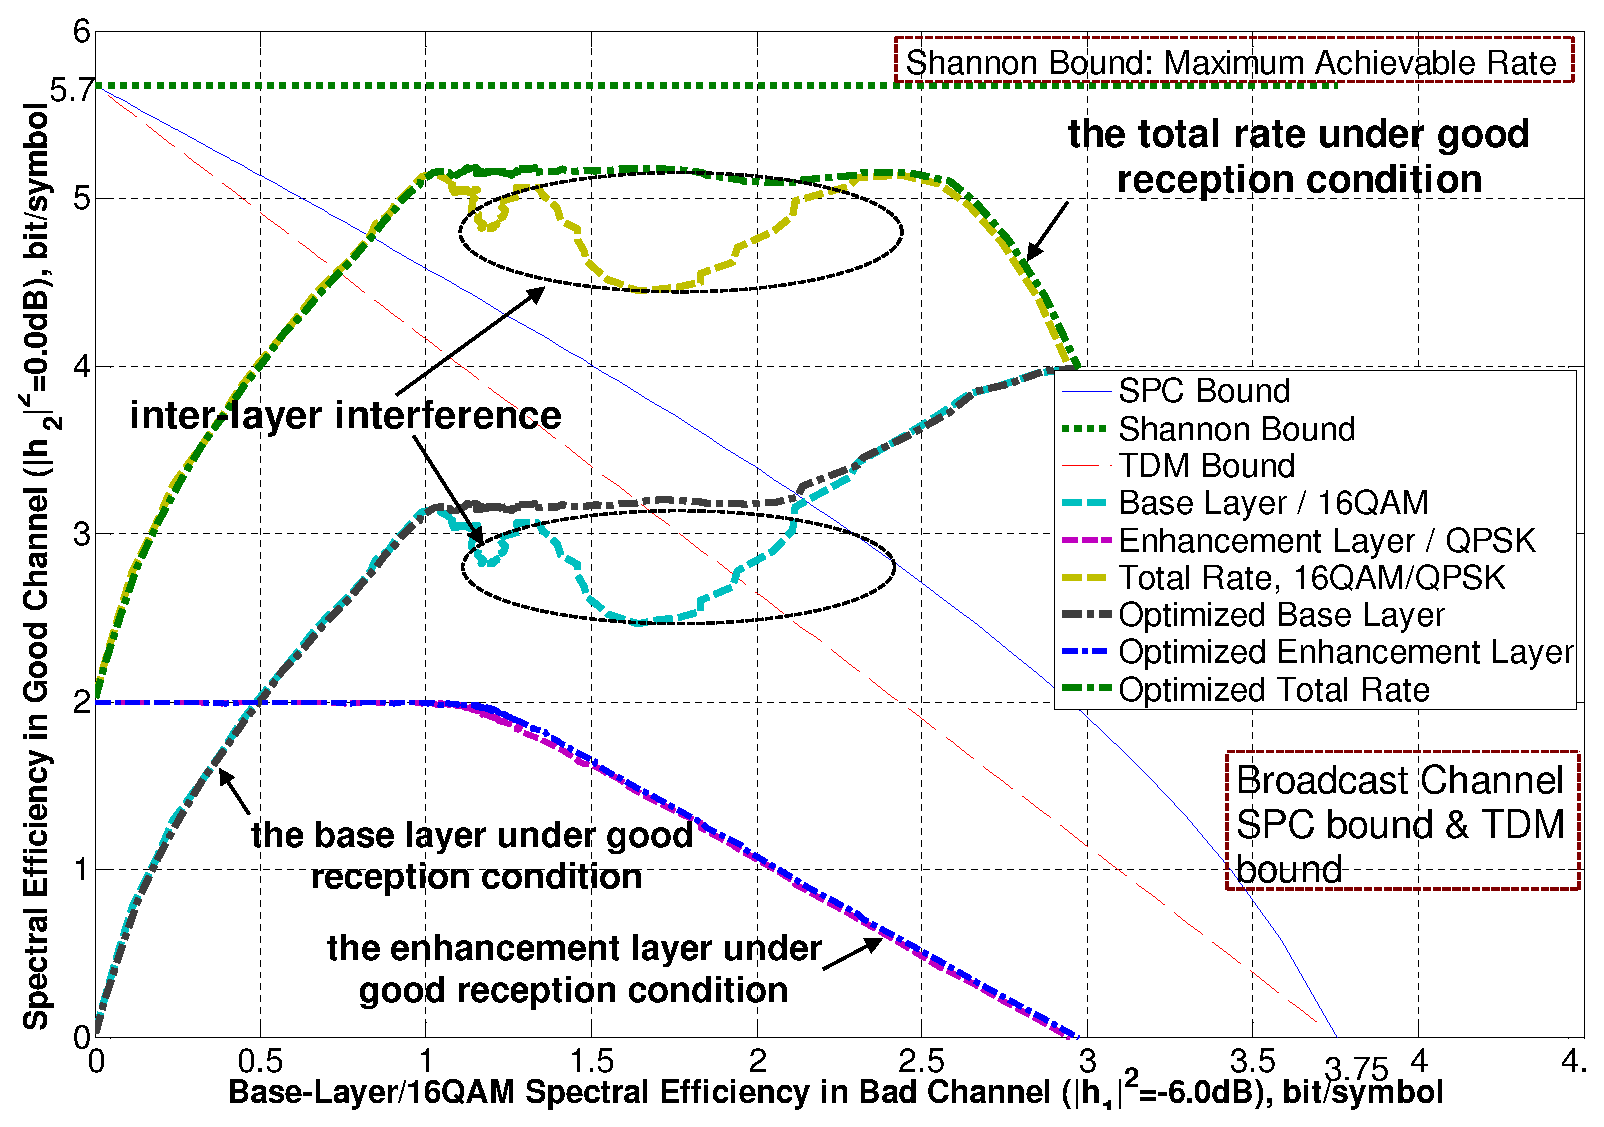
\includegraphics[width=3.0in, angle=0]{Capacity_100_025_16QAM.eps}
\caption{Achievable capacity of hierarchical modulations with
16QAM base layer and QPSK enhancement layer.}\label{Sum_Capacity}
}
\end{figure}
Hierarchical modulation is a signal precoding technique for
multiplexing multiple data streams into single symbol stream in
which each symbol consists of one base layer and one or multiple
enhancement layers. When hierarchical-modulated signals are
transmitted, users with good reception and advanced receiver can
demodulate multiple layers while others with conventional receiver
or poor reception may only demodulate the data stream embedded in
base layer. Therefore network operator can target different types
of users with different services or QoS. But traditional
hierarchical modulation may suffer from serious inter-layer
interference (ILI) so that the achievable rate by low-layer
signal(s), e.g. base-layer signals, is dented by interference from
high-layer signal(s). One example of this is shown in Fig.
\ref{Sum_Capacity}, where the 16QAM-modulated base layer suffers
from the existence of QPSK-modulated enhancement layer. In order
to recover the capacity loss due to the interference from
enhancement layer(s), two approaches are presented in this paper.
One approach is to optimize the signal constellation of
enhancement layer(s) so that higher throughput is achievable when
demodulating low-layer signals. The other one is to extend
traditional single-layer Gray bits-to-symbol mapping to
multi-layer Gray mapping for minimizing bit-error rates (BER). In
Fig. \ref{Sum_Capacity}, it shows that the rate loss by regular
hierarchical modulation can be restored by using the proposed
schemes. Another important advantage of the proposed schemes is
the incurred implementation complexity increase is low. Partial of
our schemes is adopted in UMB by 3GPP2~\cite{UMB}.
\section{Sinal Model And Problem Description}
We will limit our discussions to two-layer signal constellations
with the enhancement layer QPSK-modulated and the base layer QPSK-
or 16QAM-modulated in this paper, although the concepts proposed
here can be generalized to most hierarchical modulations. The
reason for this is not only because of the simplicity of QPSK and
16QAM modulations but also because QPSK and 16QAM are of the most
popular signal constellations adopted in various digital
communication systems and standards. It is also shown that the
addition of QPSK as enhancement layer may yield significant
performance gain by using our approaches. Since many high-order
regular or hierarchical signal constellations may be decomposed
into multiple QPSK signals adding together, many analysis and
conclusions presented in this paper can be straightforwardly
extended.

The signal constellations of regular square-shaped QPSK/QPSK and
16QAM/QPSK hierarchical modulation are shown in Fig.
\ref{regular_hierarchical}~\footnote{In this paper, a hierarchical
modulation is denoted by {\em layer 0 (or base layer)
constellation / layer 1 constellation / \ldots}, where the signal
constellation of different layers are separated by backslash from
the lowest layer (also called base layer ) to the highest layer.
}. Obviously, the regular 16QAM can be taken as a special case of
QPSK/QPSK hierarchical modulation, in which both base layer and
enhancement layer are QPSK-modulated. The minimum Euclidean
distance (MED) of base layer and enhancement layer are denoted by
$2\alpha$ and $2\beta$~\footnote{Without loss of generality, it is
assumed that $\alpha\geq\beta$.}, individually. With superimposing
base-layer signal and enhancement layer signal together, the MED
of resulted hierarchical modulation becomes
\begin{equation}
\begin{array}{rcccl}
d_{\rm min}& = & \min\left\{2\left(\alpha-\beta\right),\ 2\alpha,\
2\beta\right\}&<& 2\alpha
\end{array}.\label{Regular_MED}
\end{equation}
\begin{figure}
\center{
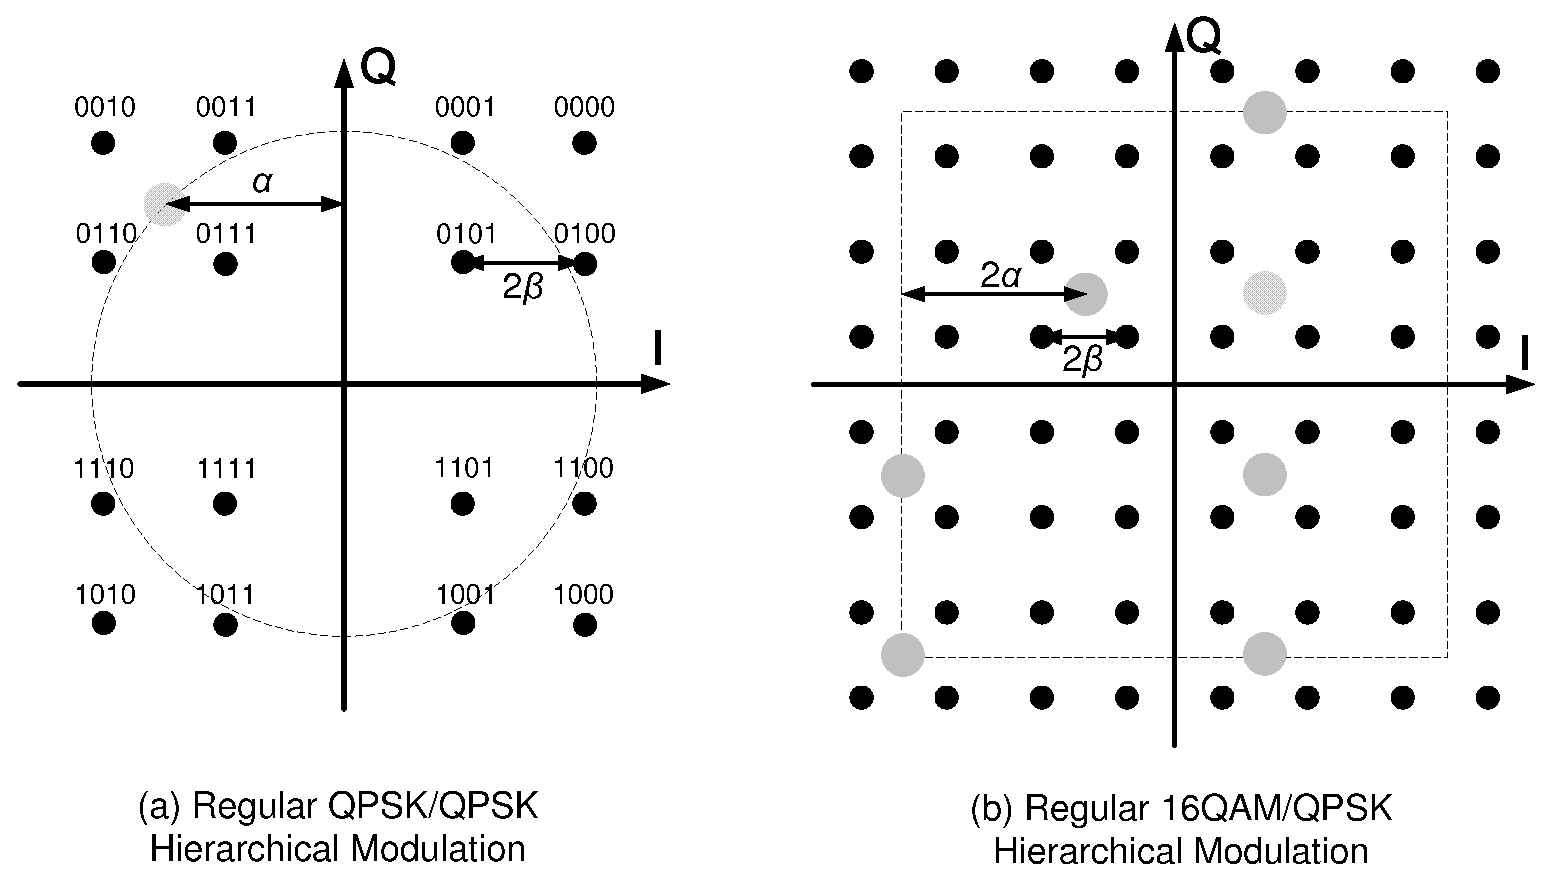
\includegraphics[width=3.0in, angle=0]{Regular_Hierarchical.eps}
\caption{Regular hierarchical modulation examples: the base layer
is QPSK/16QAM and the enhancement layer is
QPSK.}\label{regular_hierarchical} }
\end{figure}
\noindent Smaller minimum Euclid distance usually results in more
ambiguity and more demodulation errors. For demodulation BER,
another important fact is the employed bits-to-symbol mapping
rule. The bits-to-symbol mapping for hierarchical modulation shown
in Fig.~\ref{regular_hierarchical} is a interleaved Gray mapping,
where the bits $b_{0}b_{1}$ from base layer and $e_{0}e_{1}$ from
enhancement layer are interleaved in one codeword
$b_{0}e_{0}b_{1}e_{1}$. The Gray mapping shown in
Fig.~\ref{regular_hierarchical} for hierarchical signal
constellation is a kind of one-dimension Gray mapping, in which
the bits-to-symbol mapping rules for each layer are same and
independent to each other. And it is fixed regardless the
power-splitting ratio $\zeta$ between layers, which is defined by
\begin{equation}
\begin{array}{rcl}
\zeta& = & \frac{P_{\rm E}}{P_{\rm B}}
\end{array},\label{power_ratio}
\end{equation}
\noindent with $\zeta < 1$ in most cases; Otherwise we think two
signal constellations exchanged layers in hierarchical signal
constellation. For QPSK/QPSK hierarchical modulation, the
power-splitting ratio is $\zeta_{\mbox{\tiny QPSK/QPSK}}=
\frac{\beta^{2}}{\alpha^2}$. For 16QAM/QPSK modulation,
$\zeta_{\mbox{\tiny 16QAM/QPSK}}= \frac{\beta^{2}}{4\alpha^2}$.
When $\zeta_{\mbox{\tiny QPSK/QPSK}}=\frac{1}{4}$, the QPSK/QPSK
modulation in Fig.~\ref{regular_hierarchical}(a) becomes
square-shaped 16QAM. In general, the enhancement-layer signal can
be taken as additional noise by base layer. At this time, most
existing conventional receivers can continue to demodulate
base-layer signals with no additional change but at a lower
signal-to-noise/interference ratio (SINR) $\hat{\gamma}$, which is
written by
\begin{equation}
\begin{array}{rcccccl}
\hat{\gamma}& = & \frac{P_{\rm B}}{P_{\rm
E}+\sigma^2}&<&\gamma&=&\frac{P_{\rm B}}{\sigma^2}
\end{array}\label{SINR}
\end{equation}
\noindent with $\sigma^2$ denoting the power of the background
additive Gaussian white noise (AWGN),  especially when $\zeta$ is
small. On the other hand, signals of both base layer and
enhancement layer(s) can be demodulated by a advanced receiver.
This is called the strictly backward compatibility of hierarchical
modulation, which makes it attractive for providing seamless
upgrading, unequal protection, additional services or
differentiated QoS with little change on existing digital
broadcast systems.

However, regular hierarchical modulation may seriously suffer from
ILI, which not only decreases the base-layer SINR from ${\gamma}$
to $\hat{\gamma}$ but also lowers the achievable spectral
efficiency. This is observed from Fig.~\ref{Sum_Capacity}. On the
other hand, it is well-known that the achievable throughput of a
received signal essentially depends on the power distribution
profile of the signal~\cite{Unge82} in signal space instead of the
power-splitting ratio $\zeta$. This is similar to channel coding.
From a channel coding point of view, higher throughput is
achievable by the {\em i.i.d. Gaussian code} defined in coding
space, even though it may not be implementable from an engineering
standpoint~\cite{Cover72}. How to transmit a signal close to
Shannon channel capacity and implementable in a relatively easy
way is not only critical for the signal constellation design block
but also every other component in a communication system.
\section{The Enhanced Hierarchical modulations}
In order to minimize ILI effects for higher achievable throughput,
we propose two approaches for enhancing regular hierarchical
modulations, e.g., the ones shown in
Fig.~\ref{regular_hierarchical}. The description of the approaches
are presented in this section.  We will detail and discuss the
rationales behind these two approaches in the following several
sections. Computer simulations are provided along with
discussions.

The first approach is to optimally rotate the enhancement-layer(s)
of a signal constellation. For the QPSK/QPSK hierarchical
modulation shown in Fig.~\ref{regular_hierarchical}(a), the QPSK
signal constellation of the enhancement layer is rotated in the
anti-clock direction by $\theta$, $0\leq\theta\leq\frac{1}{4}\pi$,
and resulted signal constellation is shown in Fig.
\ref{enhanced_hierarchical}(a). For 16QAM/QPSK, the regular and
enhanced hierarchical modulations are shown in
Fig.~\ref{regular_hierarchical}(b) and Fig.
\ref{enhanced_hierarchical}(b), respectively.  With optimal
rotation angle $\theta_{\rm opt}$, most of the lost base-layer
capacity can be recovered without scarifying the throughput of
enhancement layer(s). As shown in Fig.~\ref{Sum_Capacity}, the
achievable rate of QPSK-modulated enhancement layers is unchanged
before and after the rotation.
\begin{figure}
\center{
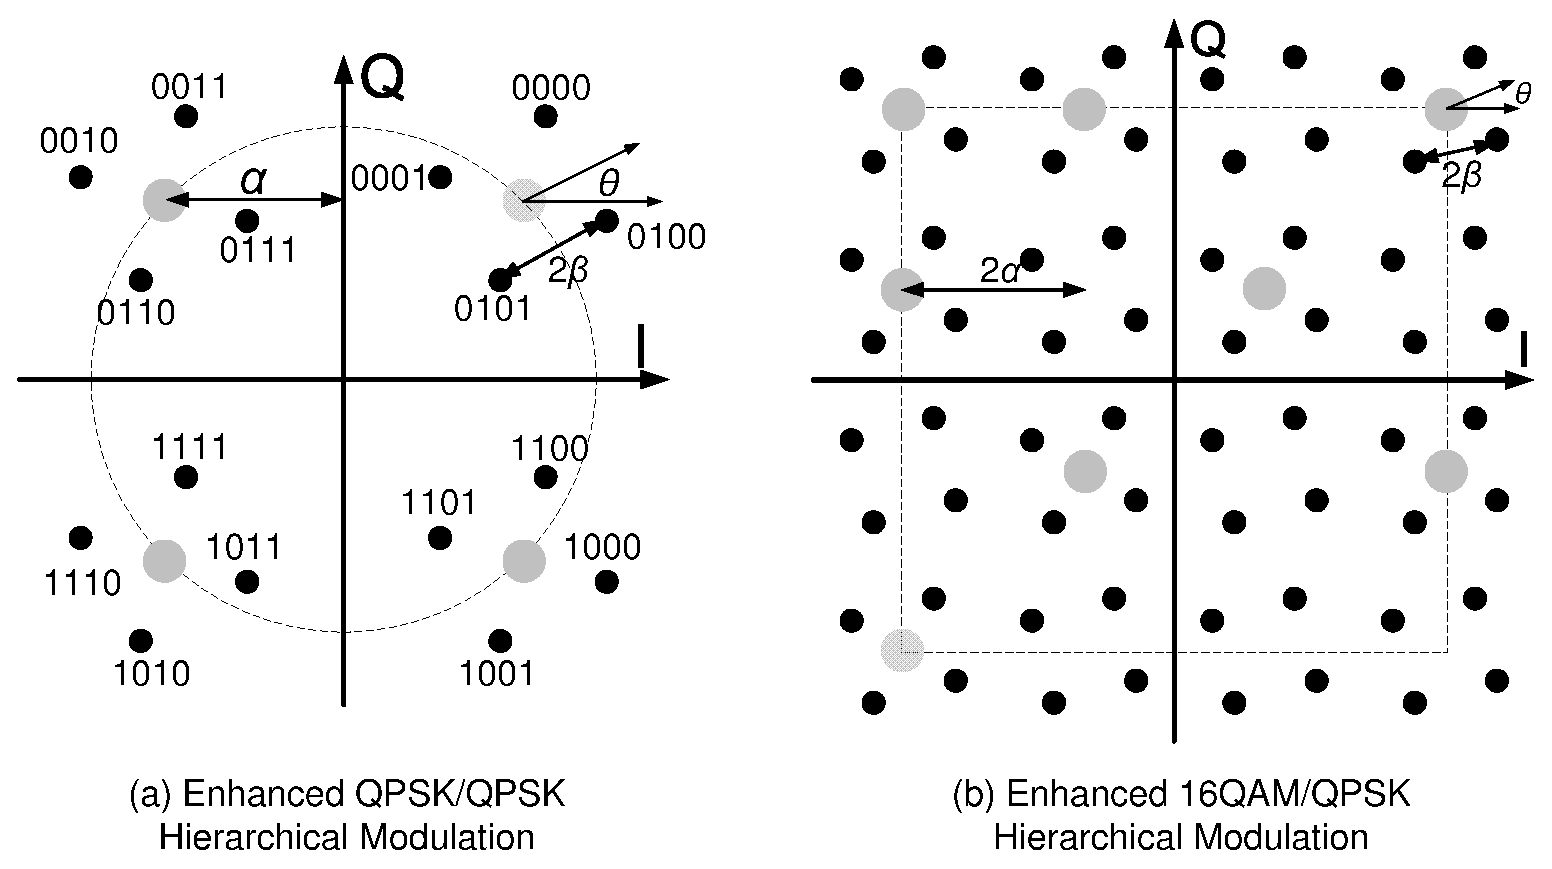
\includegraphics[width=3.0in, angle=0]{Enhanced_Hierarchical.eps}
\caption{Enhancing hierarchical modulation by rotating enhancement
layer.}\label{enhanced_hierarchical} }
\end{figure}

In reality, most capacity-achieving codes are designed to balance
the implementation complexity and achievable performance. Gray
codes is one of the examples of this. Gray code, also known as
reflective binary code, is a binary numeral system where two
successive value differ in only one digit. Even though it was
original designed to prevent spurious output from
electromechanical switches, Gray code for bits-to-symbol mapping,
mostly called Gray mapping and being implemented with other
channel coding, is generally accepted as the optimal mapping rule
for minimizing BER. Gray mapping for regular QPSK/QPSK
hierarchical modulation can be found in
Fig.~\ref{regular_hierarchical}, where the codewords with minimum
Euclid distance have minimum Hamming distance as well. However,
the Euclid distance profile will change when the enhancement-layer
signal constellation is rotated and the power-splitting ratio is
changed. This means the original Gray mapping in
Fig.~\ref{regular_hierarchical} may not always be optimal. In this
case, it may be necessary to do bits-to-symbols remapping based on
each Euclidean distance file instance. One example of Gray
remapping for QPSK/QPSK hierarchical modulation is shown in Fig.
\ref{Gray_remapping}, in which the bits-to-symbol mapping is
re-arranged when the inter-layer MED is enough smaller.
\begin{figure}
\center{
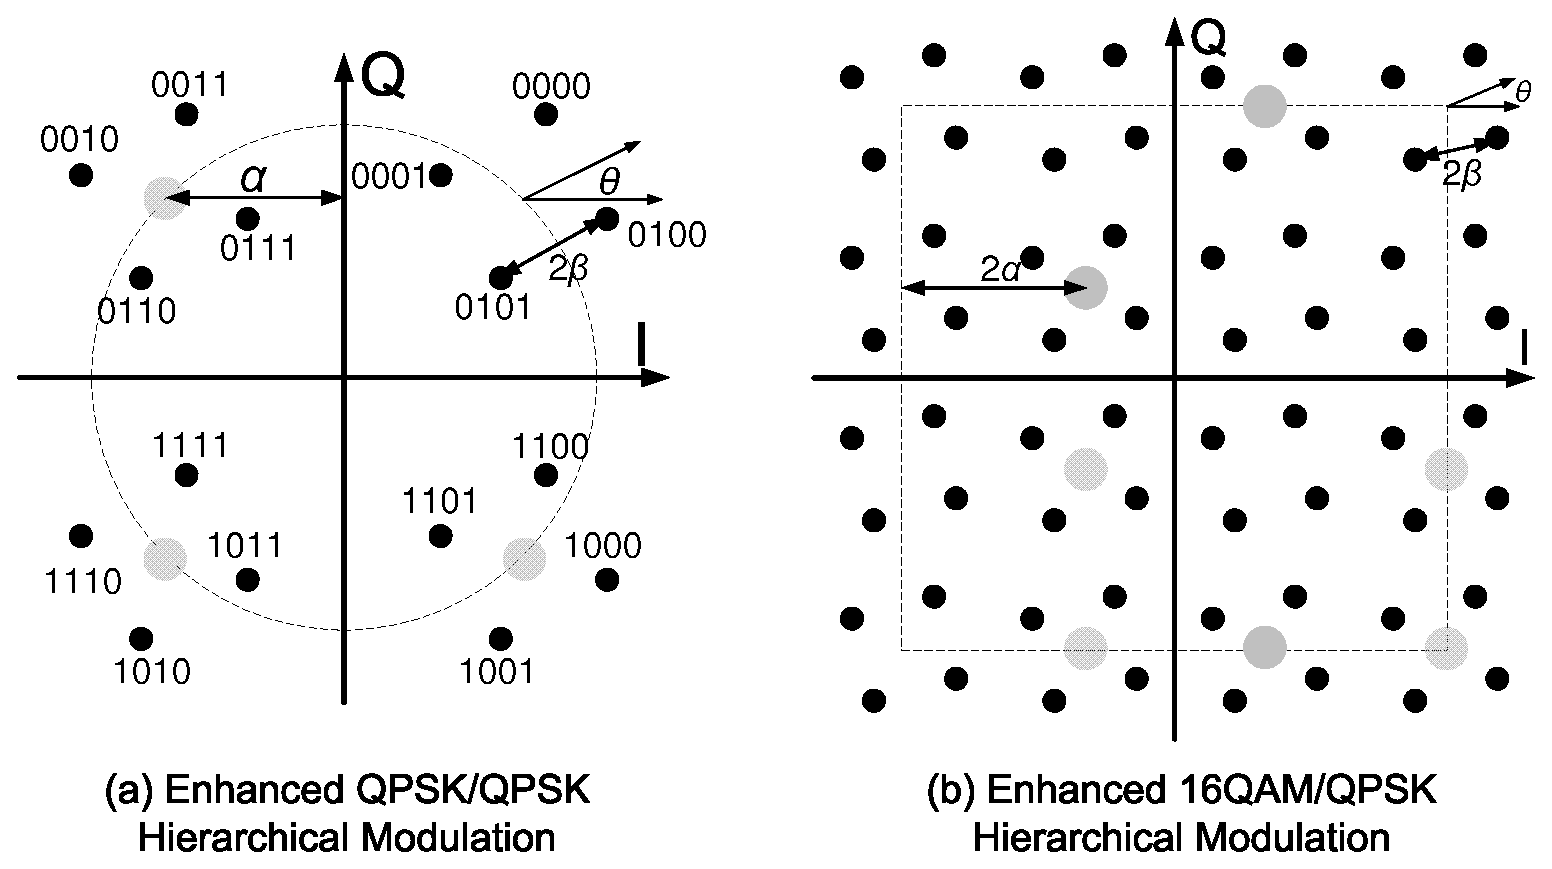
\includegraphics[width=3.0in, angle=0]{Gray_Remapping2.eps}
\caption{Enhancing hierarchical modulation by multi-dimension Gray
mapping when $2\beta>\max\left\{\Delta_{1},\
\Delta_{2}\right\}$}\label{Gray_remapping} }
\end{figure}
\section{Achievable Rate of Modulated Signals~\label{Info_Theory}}
More three decades ago Cover showed that higher sum capacity is
achievable if messages for two users of different reception
conditions are superpositedly precoded~\cite{Cover72}.
Hierarchical modulation is one of the practical implementations of
superposition precoding (SPC) for providing different rates and
protections for users with different receptions. In general, the
achievable rate of a $N$-ary modulated signal, either of regular
signal constellation or of hierarchical signal constellation,
through AWGN channel is given by~\cite{Unge82}
\begin{equation}
\begin{array}{lcl}
R&=&\log_{2}\left(N\right)-\\
&&\hspace{-0.20in}\frac{1}{N}\sum\limits_{i=0}^{N-1}\mbox{E}\left\{\log_{2}\left[\sum\limits_{j=0}^{N-1}e^{-\frac{\left|s_{j}+n-s_{i}\right|^2-\left|n\right|^2}{2\sigma^2}}\right]\right\}\
,
\end{array}\label{N_ary}
\end{equation}
\noindent which is the achievable rate when a receiver try to
decode the whole hierarchically modulated symbol. With
(\ref{N_ary}), the AWGN capacity of regular QPSK and 16QAM can be
plotted as in Fig \ref{capacity_16QAM}. Though the rate in
(\ref{N_ary}) is achievable by users with advanced receiver, it is
more than achievable for a user with a conventional demodulation
receiver which usually detects the base-layer signals only. The
achievable rate of either base layer or enhancement layer is lower
than (\ref{N_ary}). Following the concept of the successive
interference cancellation, the achievable rate, also termed {\em
equivalent capacity}, for a receiver decoding up to $l$ layers of
a hierarchical modulated symbol is~\cite{Huber94}
\begin{equation}
\begin{array}{rcccl}
\tilde{R}_{l}&=&\sum\limits_{i=0}^{l-1}R_{i}& = &
R-\sum\limits_{j=l}^{L}{R}_{j}
\end{array}.\label{R_equiv}
\end{equation}
\noindent Let's take the regular 16QAM as an example. A regular
16QAM can be take as a special case of QPSK/QPSK hierarchical
modulation with $\zeta_{\mbox{\tiny QPSK/QPSK}}=\frac{1}{4}$. This
means the achievable rate of the enhancement layer is the same as
the regular QPSK capacity and the achievable rate of the base
layer becomes
\begin{equation}\hspace{-0.2in}
\begin{array}{rl}
{\rm R}_{\mbox{\tiny QPSK/QPSK}}^{\rm B}\left(\gamma,\
\frac{1}{5}\right)&\hspace{-0.08in}=\ {\rm R}_{\mbox{\tiny
QPSK/QPSK}}\left(\gamma,\
\frac{1}{5}\right)-{\rm R}_{\mbox{\tiny QPSK}} \left(\frac{1}{5}\gamma\right)\\
&\hspace{-0.08in}=\ {\rm R}_{\mbox{\tiny
16QAM}}\left(\gamma\right)-{\rm R}_{\mbox{\tiny
QPSK}}\left(\frac{1}{5}\gamma\right)\ ,
\end{array}\label{R_16QAM_B1}
\end{equation}
\noindent when are plotted in Fig \ref{capacity_16QAM}. Due to the
ILI from the QPSK-modulated enhancement layer, the actual
throughput of the QPSK base layer ${\rm R}_{\mbox{\tiny
QPSK/QPSK}}^{\rm B}\left(\gamma,\ \frac{1}{5} \right)$ is lower
than the corresponding QPSK rate ${\rm R}_{\mbox{\tiny
QPSK}}\left(\frac{4}{5}\gamma\right)$, i.e.,
\begin{equation}
\begin{array}{rcl}
{\rm R}_{\mbox{\tiny QPSK/QPSK}}^{\rm B}\left(\gamma,\ \frac{1}{5}
\right)&\leq&{\rm R}_{\mbox{\tiny QPSK}}
\left(\frac{4}{5}\gamma\right)
\end{array}.\label{R_16QAM_B2}
\end{equation}
\begin{figure}
\center{
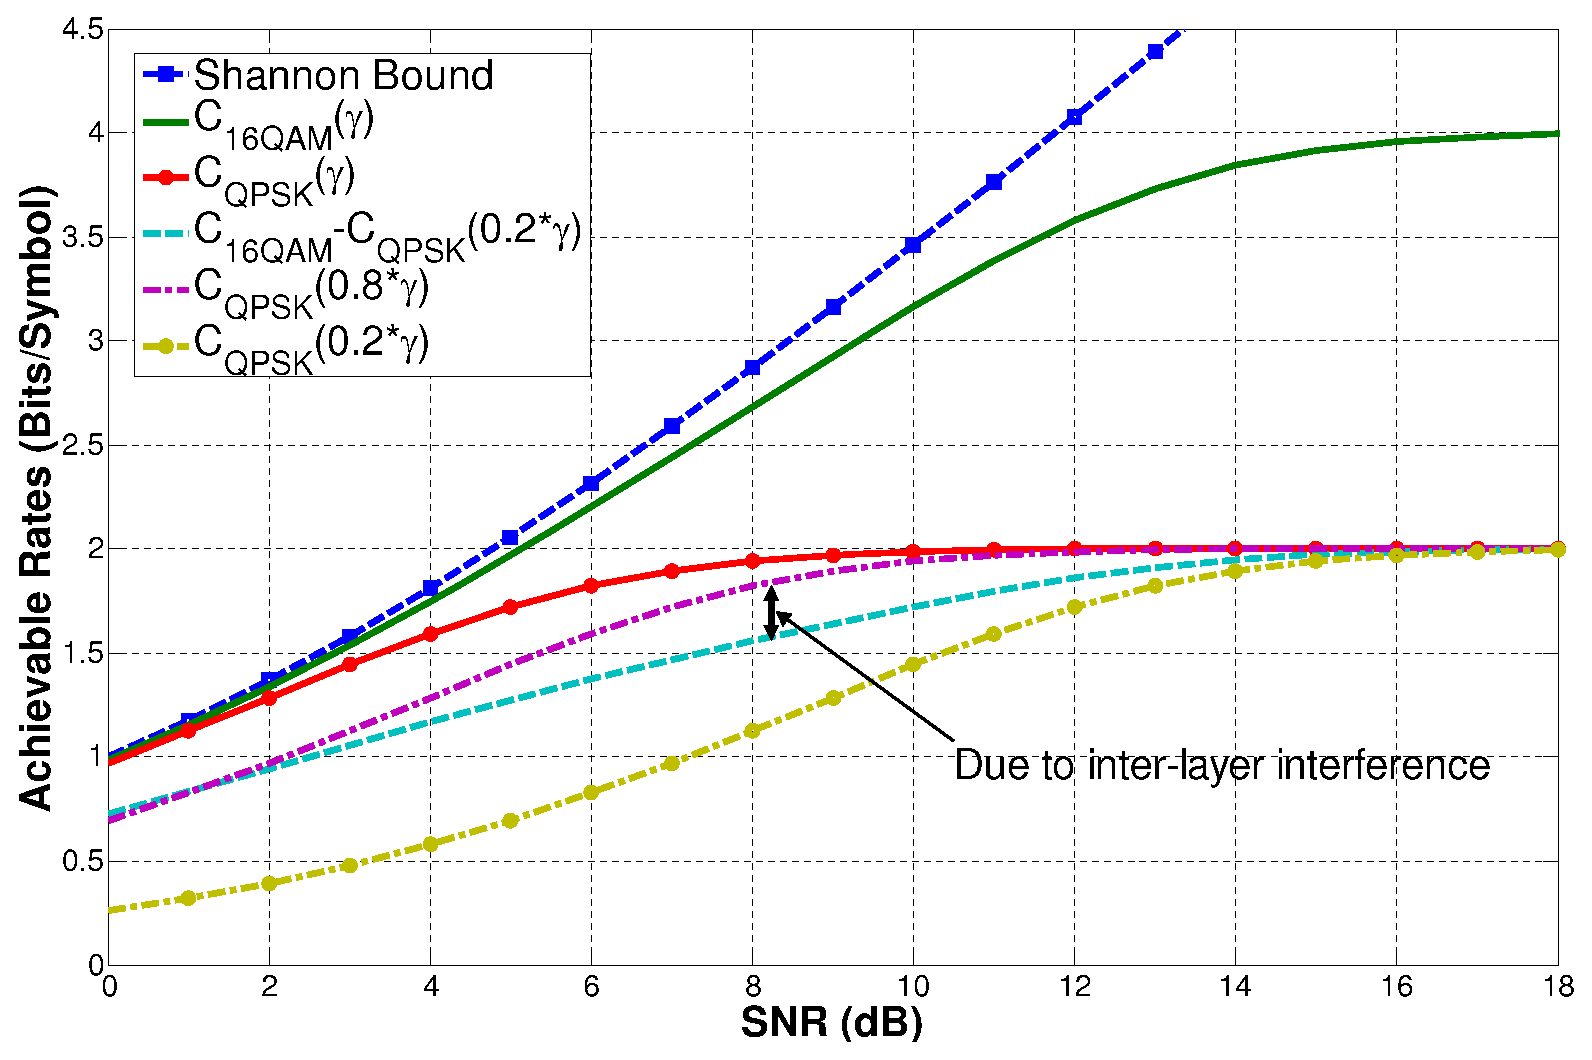
\includegraphics[width=3.0in, angle=0]{Capacity_16QAM.eps}
\caption{Achievable rates of regular 16QAM modulation: a
hierarchical modulation perspective.}\label{capacity_16QAM} }
\end{figure}
\noindent In Fig \ref{capacity_16QAM}, it shows that the
degradation of the base-layer capacity can be up to around
$\Delta=0.56$ bits/symbol, which is about $14\%$ of the maximum
total achievable rate $2$ bits/symbol for the QPSK base-layer.
This kind of degradation can be further illustrated in
Fig.~\ref{capacity_rotating}, where the hierarchical modulation is
16QAM/QPSK-modulated. In Fig.~\ref{capacity_rotating}, the total
SNR is fixed at $\frac{P}{\sigma^2}=20\mbox{dB}$ but the power of
the 16QAM sublayer is changed from $0\%$ to $100\%$ of the total
power $P$. The achievable rates of each layer and the whole
constellation are plotted in Fig.~\ref{capacity_rotating}. One of
the interesting things shown in Fig. \ref{capacity_rotating} is
the equivalent capacity of the 16QAM base layer changes
periodically instead of monotonically with increase the power
ratio between the base layer and the whole signal. The good things
in Fig. \ref{capacity_rotating} is this kind of capacity loss can
be recovered by optimally rotating the enhancement layer. This is
one of the advantages of the proposed enhanced hierarchical
modulations.
\begin{figure}
\center{
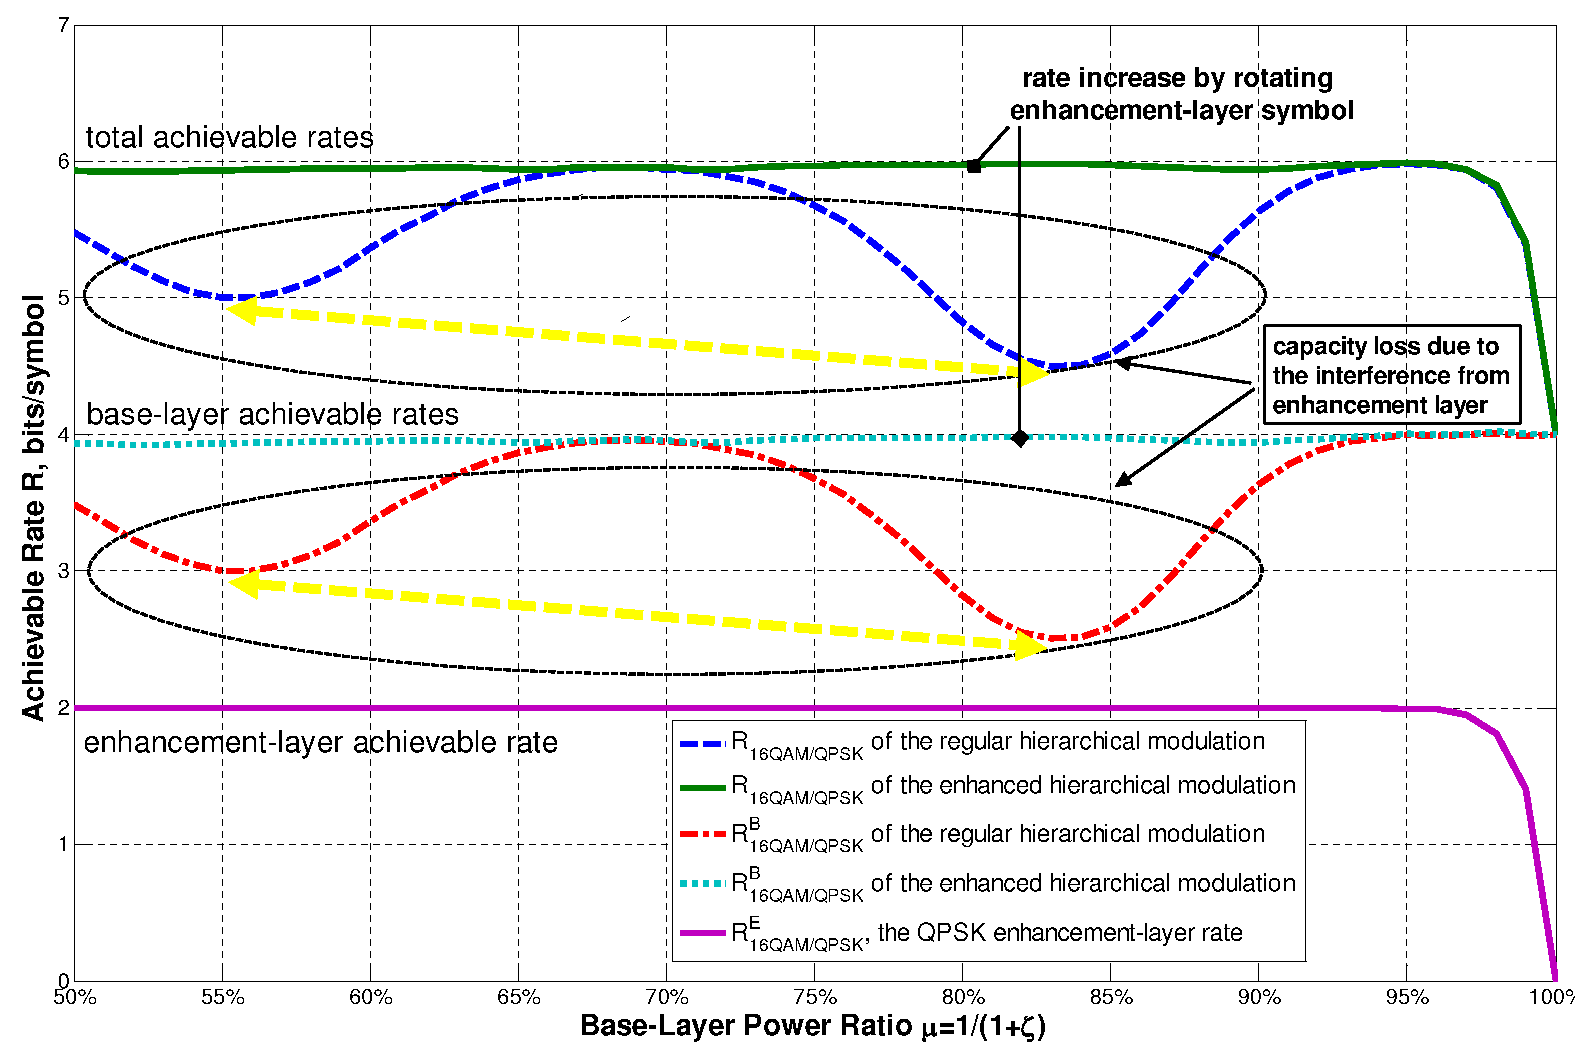
\includegraphics[width=3.0in, angle=0]{Capacity_power_splitting.eps}
\caption{Achievable rates of 16QAM/QPSK hierarchical modulation
with different power splitting and
$\frac{P}{\sigma^2}=20$dB.}\label{capacity_rotating} }
\end{figure}
\section{Effective Signal-to-Noise Ratio and Modulation Efficiency}
Besides the above information-theoretical point of view of
hierarchical modulation, it is also interesting to understand
hierarchical modulation from a signal-processing perspective. At
this time, the performance of hierarchical modulation will be
evaluated through actual implementations, where demodulation BER
is one of the major concerns. In general, it is difficult to give
a simple closed-form BER expression for hierarchical signal
constellation. The BER of square-shaped $M$-QAM constellation and
a hierarchical QAM constellation can be computed by using
recursive algorithms~\cite{Vitt03}. It is known that the BER
expression for QPSK is
\begin{equation}
\begin{array}{rcl}
{\rm P}_{e,\mbox{\tiny QPSK}}\left(\gamma\right)&=&{\rm
Q}\left(\sqrt{\frac{\gamma}{2}}\right)
\end{array},\label{BER_QPSK}
\end{equation}
\noindent where ${\rm Q}\left(x\right)=\frac{1}{2}{\rm
erfc}\left(\frac{x}{\sqrt{2}}\right)$ denotes the $\rm
Q$-function.
\begin{figure} \center{
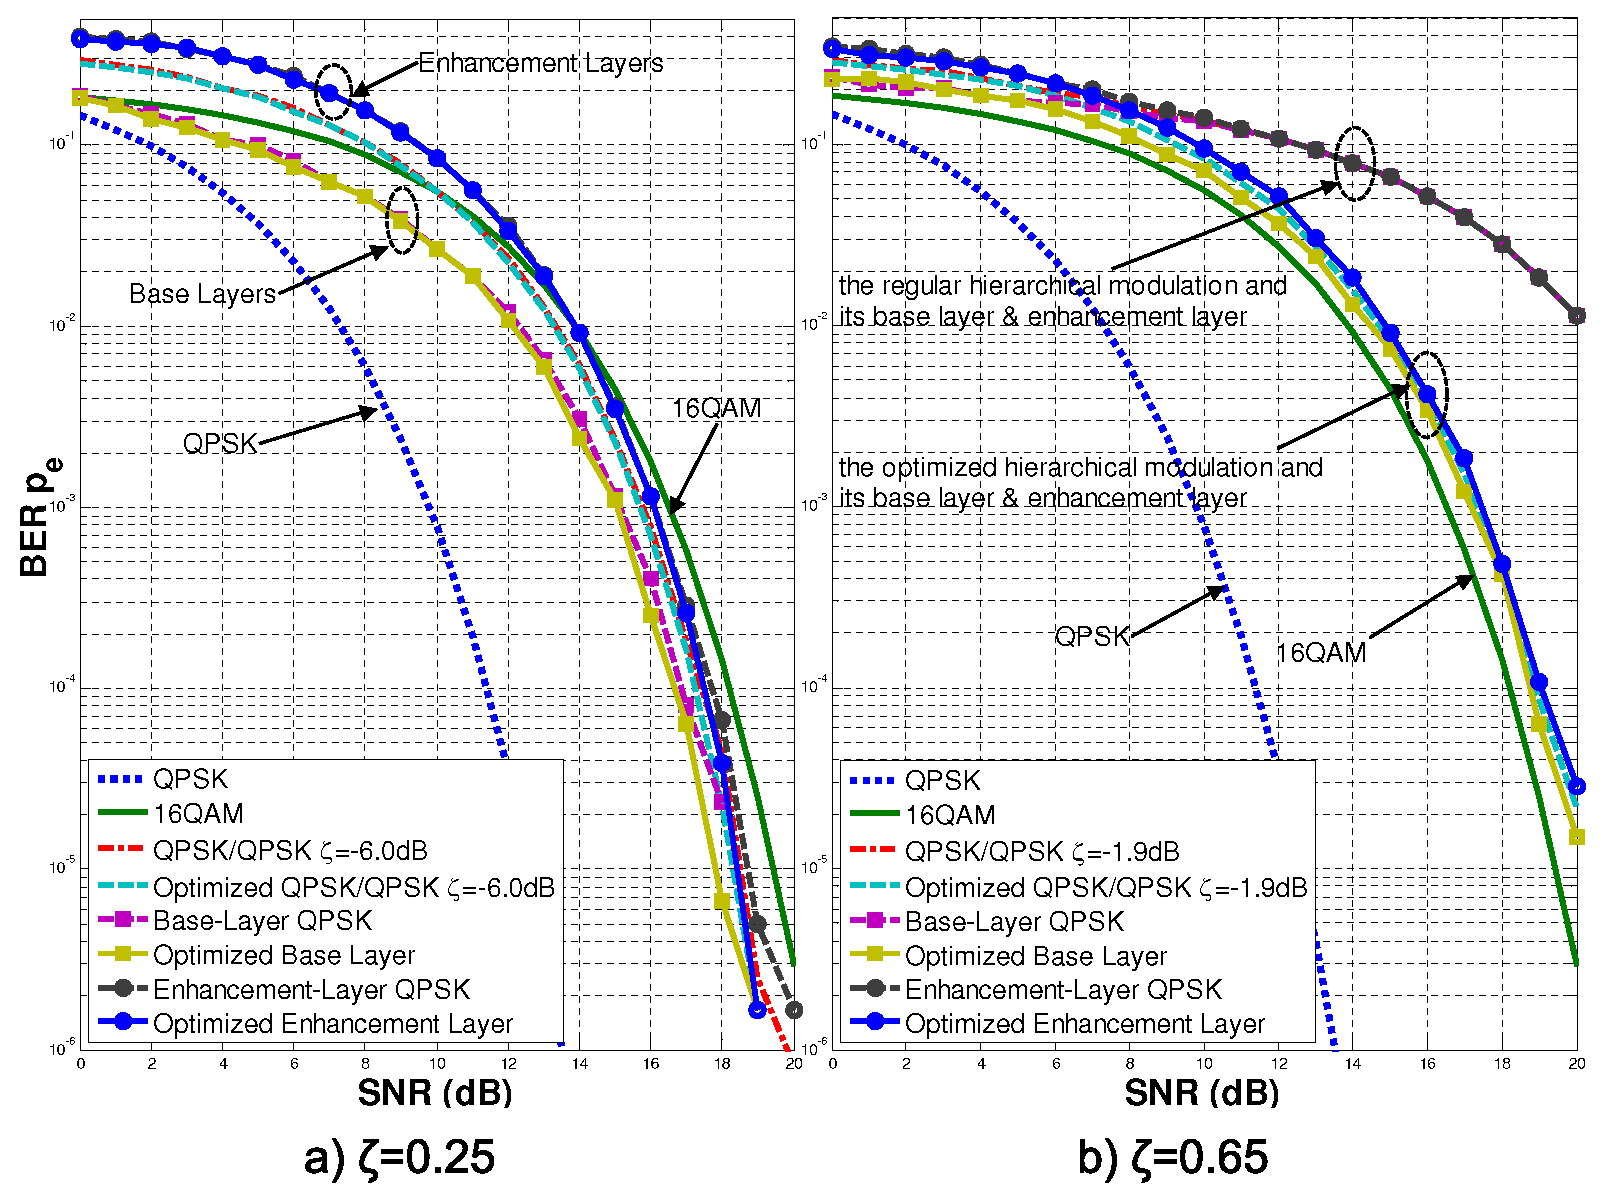
\includegraphics[width=3.20in, angle=0]{BER_Hierarchical.eps}
\caption{Bit-error rate of uncoded QPSK/QPSK hierarchical
modulations using maximum likelihood demodulation . } \label{BER}}
\end{figure}
From a signal processing standpoint, the BER and capacity
degradation may happen when there is a change in noise and/or
interference distribution, even though the received SNR $\gamma$
is the same. For example, the BER performance of regular QPSK/QPSK
hierarchical modulation becomes deteriorated in Fig. \ref{BER}
with increasing $\zeta_{\mbox{\tiny QPSK/QPSK}}$. But, if we
optimally rotate the enhancement-layer signal constellation, the
performance loss can be recovered. This kind of recovery can be
more significant with large $\zeta$. There are many ways for
quantifying and understanding this kind of BER performance loss
due to either interference or receiver design. One approach for
capturing this kind of degradation is to calculate the effective
signal-to-noise ratio (ESNR) for the receiver output, which is
defined by
\begin{equation}
\begin{array}{rcl}
\tilde{\gamma}\left(\gamma\right)&\equiv&\Psi^{-1}\left(p_{e}(\gamma)\right)
\end{array},\label{eff_SNR}
\end{equation}
\noindent where $p_{e}(\gamma)$ is the demodulation BER of the
signal with SNR $\gamma$ and $\Psi^{-1}\left(\ast\right)$ denotes
the inverse function of $\Psi\left(\cdot\right)$, the demodulation
error probability function with no ILI. For example, the ESNR for
the QPSK-modulated base layer or enhancement layer of any
hierarchical modulation can be calculated by
\begin{equation}
\begin{array}{rcl}
\tilde{\gamma}_{\mbox{\tiny QPSK/QPSK}}&=&2\left[{\rm
Q}^{-1}\left(p_{e}(\gamma)\right)\right]^2
\end{array}.\label{eff_SNR_QPSK}
\end{equation}
\noindent More specifically, the ESNR for the base layer of
regular QPSK/QPSK hierarchical modulation with maximum likelihood
demodulator is given by
\begin{equation}\hspace{-0.225in}
\begin{array}{l}
\tilde{\gamma}_{\mbox{\tiny QPSK/QPSK}}^{\rm
B}(\gamma)=2\left[{\rm Q}^{-1}\left(\frac{{\rm
Q}((1-\sqrt{\zeta})\gamma)+{\rm
Q}((1+\sqrt{\zeta})\gamma)}{2}\right)\right]^2.
\end{array}\label{eff_SNR_QPSK_QPSK}
\end{equation}
\noindent By normalizing ESNR by $\gamma$, we can obtain
hierarchical modulation efficiency (ME) $\eta$ by
\begin{equation}
\begin{array}{rcccl}
\eta\left(\gamma\right)&=&\frac{\tilde{\gamma}}{\gamma}&=&\frac{1}{\gamma}\Psi^{-1}\left(p_{e}(\gamma)\right)
\end{array}.\label{mod_eff}
\end{equation}
\noindent Without interference, $\eta\left(\gamma\right)=1$;
Otherwise, $\eta\left(\gamma\right)<1$. $\eta$ is also the measure
of inter-layer resistance for hierarchical modulation. Higher ME
is, stronger interference-resistance the signal has. As an
example, the ME of QPSK/QPSK hierarchical modulation are plotted
in Fig. \ref{modulation_efficiency}. We can see the enhanced
hierarchical modulation has higher ME than the regular modulation.
The difference is more obvious when $\zeta$ becomes large. This
means enhanced hierarchical modulation has stronger inter-layer
interference resistance than regular hierarchical modulation.
\begin{figure}
\center{
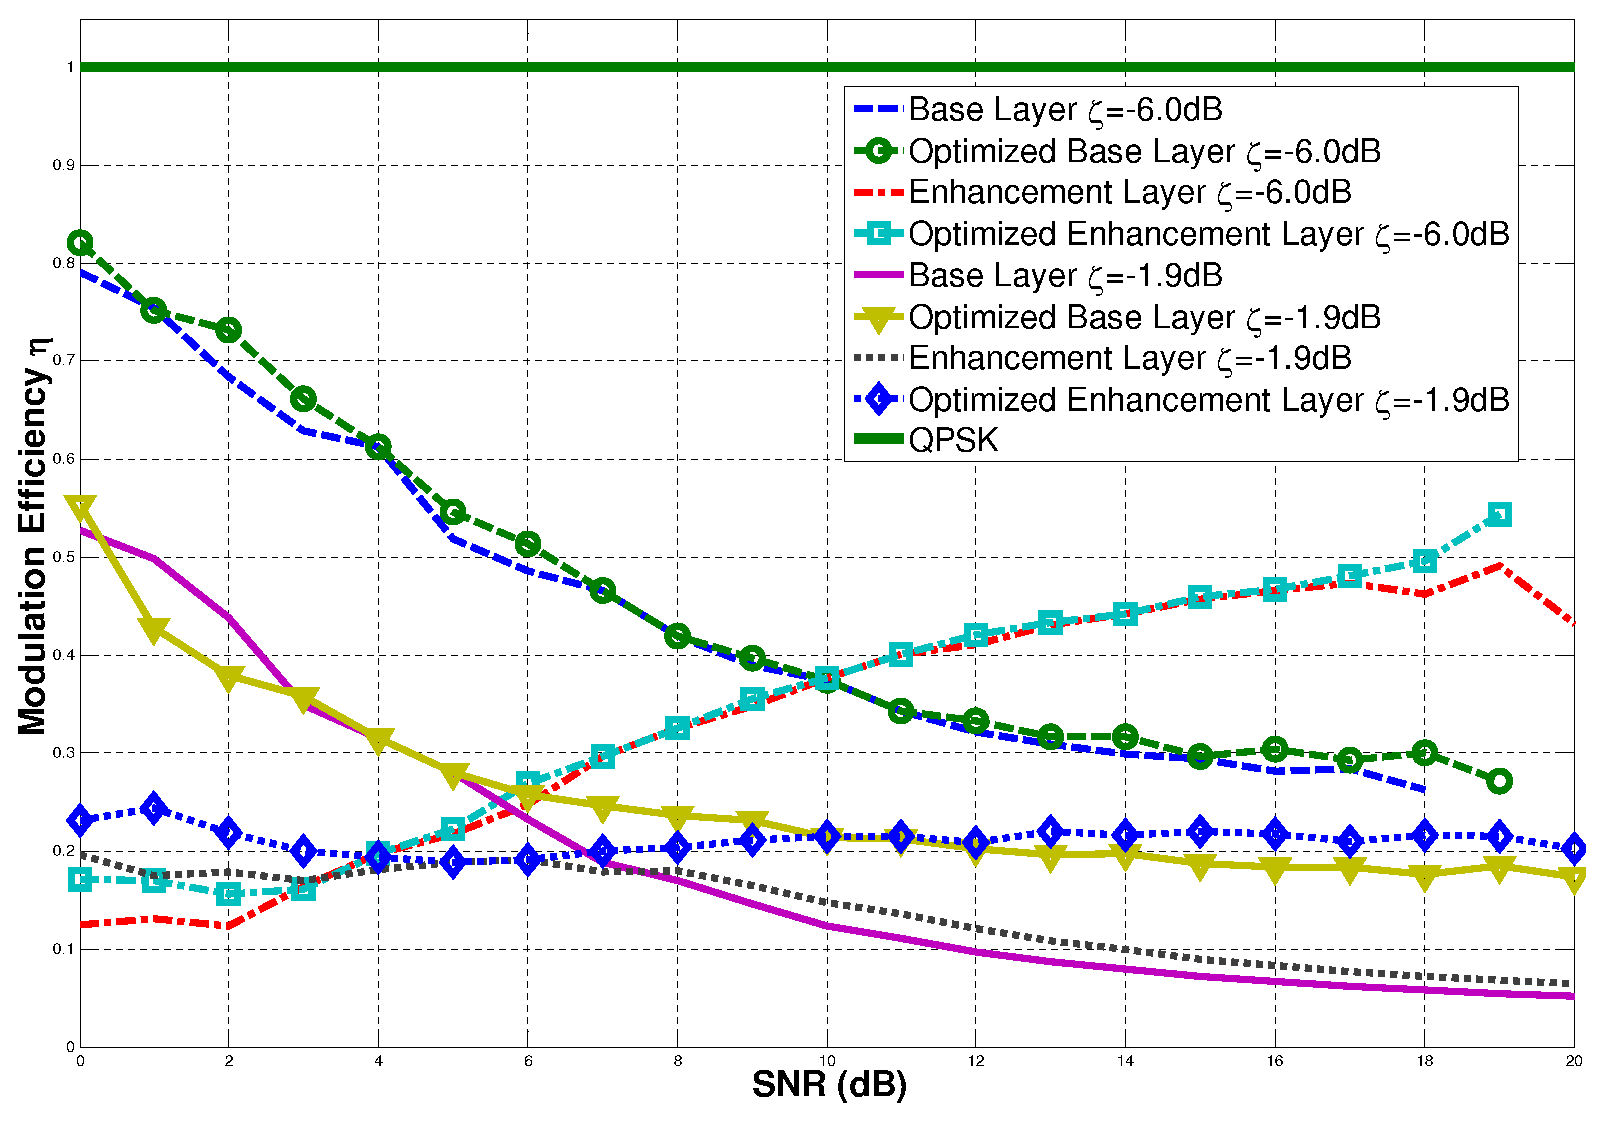
\includegraphics[width=3.0in, angle=0]{Modulation_Efficiency.eps}
\caption{Hierarchical modulation efficiency of QPSK/QPSK
hierarchical modulation using maximum likelihood
demodulation.}\label{modulation_efficiency} }
\end{figure}
\section{Asymptotic Modulation Efficiency and Voronoi Decomposition}
The asymptotic modulation efficiency (AME) $\eta_{\infty}$ is
given by
\begin{equation}
\begin{array}{rcccl}
\eta_{\infty}&=&\lim\limits_{\gamma\rightarrow\infty}\eta\left(\gamma\right)&=&\lim\limits_{\sigma\rightarrow0}\frac{\sigma^2}{P}\Psi^{-1}\left(p_{e}\right)
\end{array}.\label{asy_mod_eff}
\end{equation}
\noindent For the example in (\ref{eff_SNR_QPSK_QPSK}), the AME
can be calculated by
\begin{equation}\hspace{-0.225in}
\begin{array}{rcl}
\eta_{\infty}&=&\lim\limits_{\gamma\rightarrow\infty}\frac{2\left[{\rm
Q}^{-1}\left(\frac{{\rm Q}((1-\sqrt{\zeta})\gamma)+{\rm
Q}((1+\sqrt{\zeta})\gamma)}{2}\right)\right]^2}{\gamma}.
\end{array}\label{asy_eff_SNR_QPSK_QPSK}
\end{equation}
\noindent From (\ref{asy_mod_eff}) and
(\ref{asy_eff_SNR_QPSK_QPSK}), it shows that AME basically shows
how fast ESNR is approaching SNR when $\gamma\rightarrow\infty$.
This can be expressed by
\begin{equation}
\begin{array}{rcl}
\eta_{\infty}&=&\frac{\partial\eta\left(\gamma\right)}{\partial\gamma}|_{\gamma=\infty}
\end{array}.\label{asy_mod_eff2}
\end{equation}
\noindent The AME for QPSK/QPSK hierarchical modulation can also
be found in Fig.~\ref{modulation_efficiency}, in which they are
the points that the ME are approaching to when SNR becomes larger
and larger.

Since AME measures the effects of ILI when there is no noise, it
essentially reflects the power distribution profile of a signal
constellation in signal space, which can be further illustrated by
the Voronoi decomposition. For example, the Voronoi decomposition
for QPSK and 16QAM is show in Fig.~\ref{Voronoi_regular}, where
each Voronoi cells are rectangular. But, the Voronoi boundary for
the enhanced hierarchical modulations are different. The Voronoi
decomposition of enhanced QPSK/QPSK is shown in
Fig.~\ref{Voronoi_enhanced}, where the Voronoi boundary becomes
polygons and the area of each Voronoi region is changed. This kind
of changes certainly affect the demodulation performance of the
signals.
\begin{figure} \center{
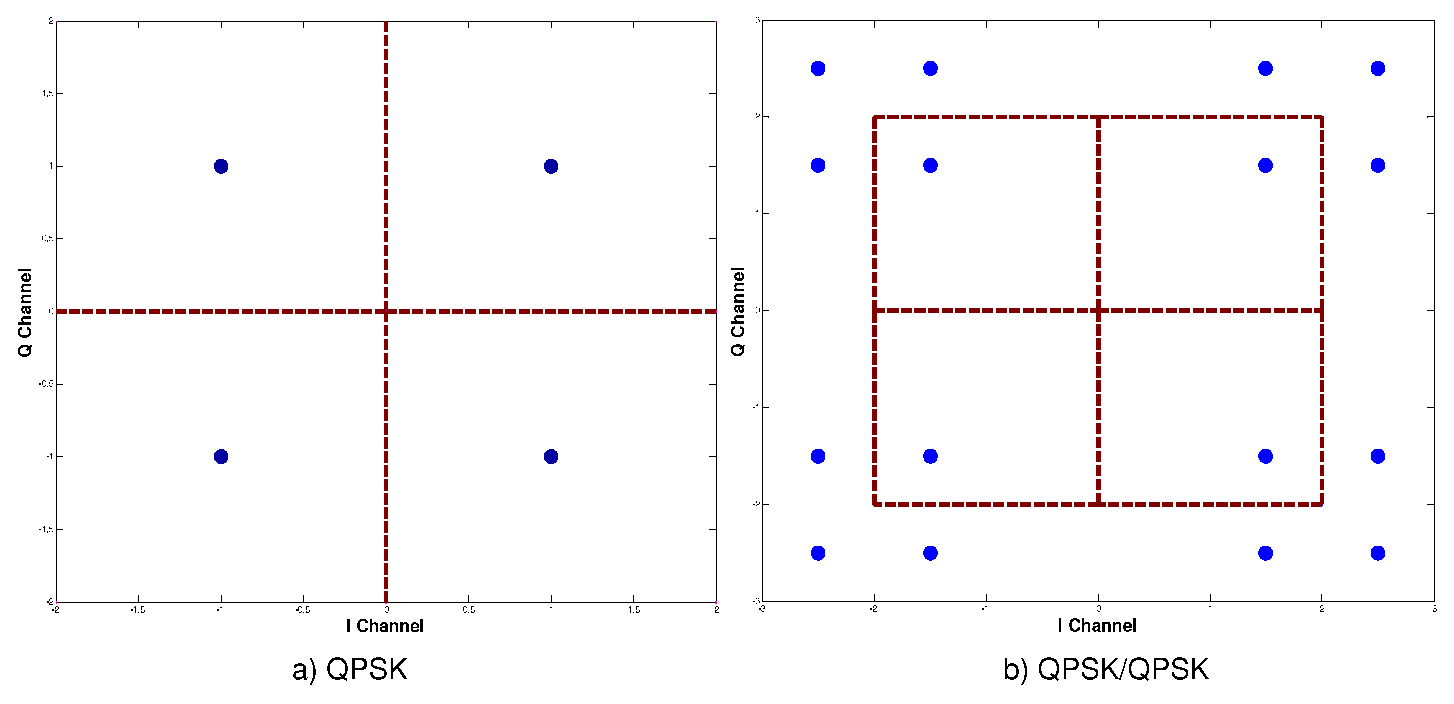
\includegraphics[width=3.20in, angle=0]{Voronoi_Regular.eps}
\caption{Voronoi diagram for regular modulations}
\label{Voronoi_regular}}
\end{figure}
\begin{figure} \center{
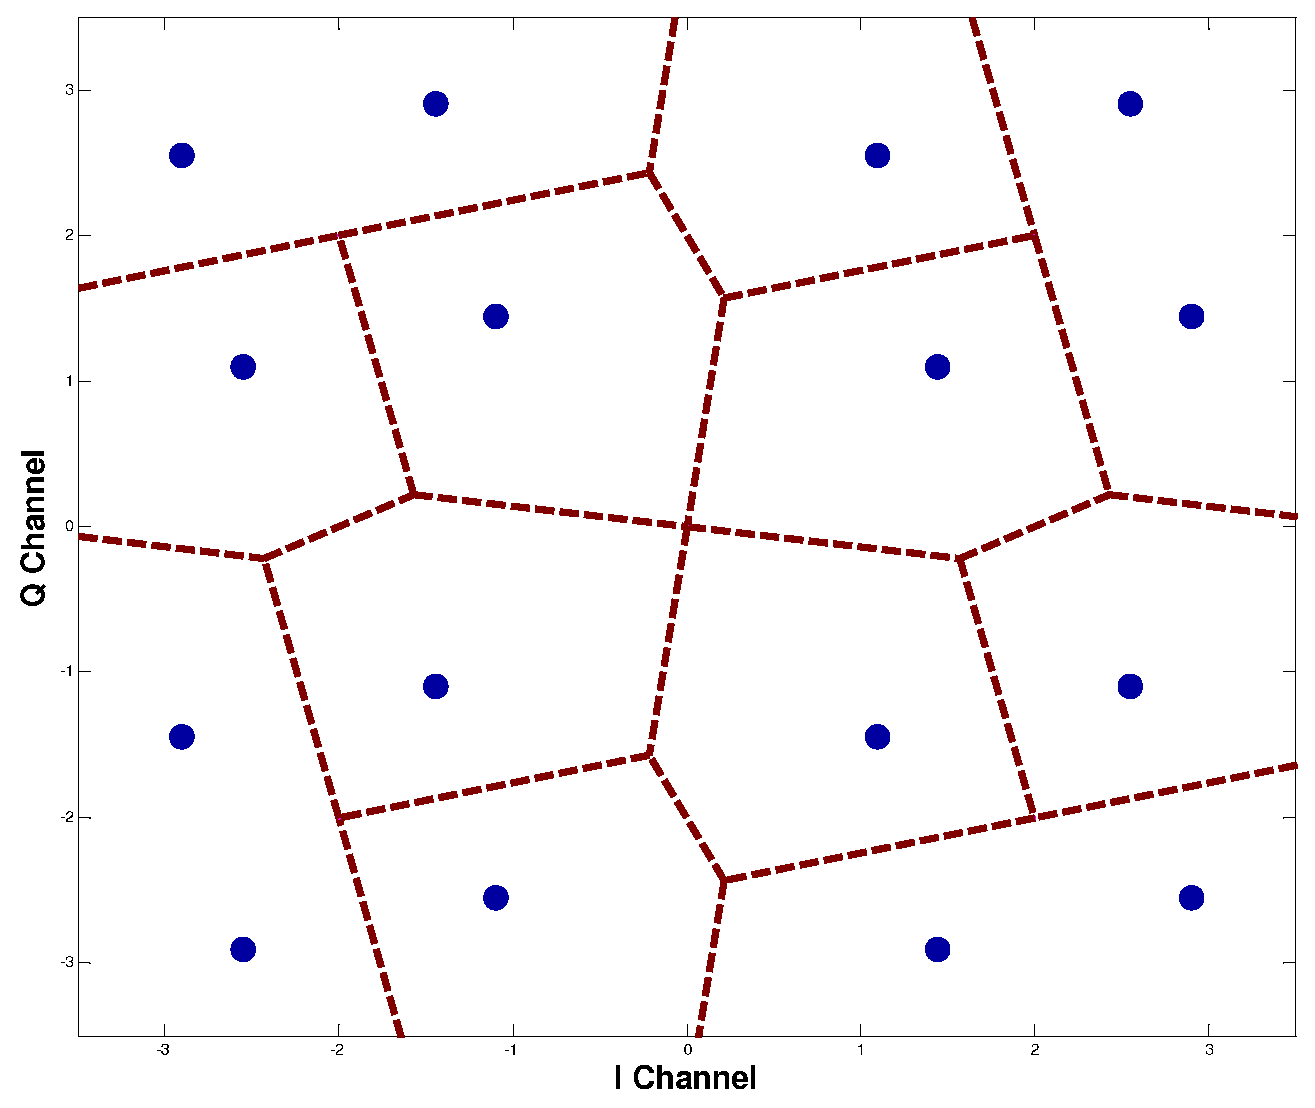
\includegraphics[width=2.40in, angle=0]{Voronoi_Enhanced.eps}
\caption{Voronoi diagram for enhanced QPSK/QPSK hierarchical
modulation} \label{Voronoi_enhanced}}
\end{figure}
\section{Euclid Distance and Hamming Distance}
When the receiver selects $\bs_i$ instead of the transmitted
symbol $\bs_j$, there is a demodulation error happened. The
demodulation error for AWGN channel is
\begin{equation}
\begin{array}{rcl}
Pr\left(\bs_{j}\rightarrow\bs_{i}|\bs_{j}\right)&=&Q\left(\frac{\|\bs_{i}-\bs_{j}\|}{\sqrt{2}\sigma}\right)
\end{array}.\label{prior_error}
\end{equation}
\noindent In a general case of Rician fading channel with Rice
factor $K$, Chernoff upper bound of
$Pr\left(\bs_{j}\rightarrow\bs_{i}|\bs_{j}\right)$ is given by
\begin{equation}
\begin{array}{ll}
\hspace{-0.2in}Pr\left(\bs_{j}\rightarrow\bs_{i}|\bs_{j}\right)&\\
&\hspace{-0.8in}\leq\
\frac{1+K}{1+K+\frac{1}{2}\gamma\|\bs_{i}-\bs_{j}\|^2}e^{-\frac{K\frac{1}{2}\gamma\|\bs_{i}-\bs_{j}\|^2}{1+K+\frac{1}{2}\gamma\|\bs_{i}-\bs_{j}\|^2}}\
.
\end{array}\label{prior_error_fading}
\end{equation}
\noindent The BER performance of a signal constellation is
dominated by symbol pairs with EMD $d_{\rm min}$ especially when
SNR is high. An example of the minimum Euclidean distance of
hierarchical distance with rotating enhancement layer can be shown
in Fig.~\ref{euclid_dist}.

In general, Gray mapping in two-dimensional signals worked with
channel coding is accepted as optimal for minimizing BER for
equally likely signals. Gray mapping for regular hierarchical
signal constellations is shown in Fig.~\ref{regular_hierarchical},
where the codes for the closest two signals are different in only
one bit. However, this kind of Euclidean distance profile may not
be fixed in hierarchical modulation. For example, when the power
splitting ratio $\zeta$ increase in a two-layer hierarchical
modulation, the inter-layer Euclidean distance between the base
layer and enhancement layer become short and the distance of some
previous closest signal pairs may be not the shortest any more.
This may also happen when the enhancement layer is rotated.
Therefore in order to minimize BER when Euclidean distance profile
is changed in hierarchical modulation, it may be necessary to do
Gray-remapping. One example of Gray remapping is shown in
Fig.~\ref{Gray_remapping}. Their BER performance is shown in Fig.
\begin{figure}
\center{
\includegraphics[width=3.0in, angle=0]{MED_16QAM_QPSK.eps}
\caption{Minimum Euclidean distance of 16QAM/QPSK
modulations}\label{euclid_dist} }
\end{figure}
\section{Conclusions}
In this paper, two schemes for enhancing hierarchical modulations
are presented for higher throughput and less error rate. One
approach is to optimize the signal constellation and the other one
is to do multi-dimensional Gray mapping. The rationale and
performance of the proposed approaches are discussed and analyzed
by calculating the achievable rate, effective signal-to-noise
ration and minimum Euclidean distance. These two approaches can be
applied for upgrading existing broadcast systems with minimum
complexity increase and designing the next-generation BCMCS
systems. Some of them is adopted in the 4th generation mobile
communication standard UMB developed by 3GPP2. \small
\bibliographystyle{unsrt}
\bibliography{Hierarchical_Modulation}
\end{document}
